\documentclass{article}
\usepackage[utf8]{inputenc}
\usepackage{mathrsfs}
\usepackage{tikz}
\usepackage{amssymb}
\usepackage{amsthm}
\usepackage{graphicx} % Required for inserting images
\usepackage{amsmath}
\usepackage{MnSymbol}
\usepackage{geometry}
\usepackage{physics}
\usepackage{enumerate}
\allowdisplaybreaks
\newcommand\numeq[1]%
  {\stackrel{\scriptscriptstyle(\mkern-1.5mu#1\mkern-1.5mu)}{=}}
\newcommand\numleq[1]
  {\stackrel{\scriptscriptstyle(\mkern-1.5mu#1\mkern-1.5mu)}{\leq}}
\newcommand\numgeq[1]
  {\stackrel{\scriptscriptstyle(\mkern-1.5mu#1\mkern-1.5mu)}{\geq}}

\newtheorem{definition}{Definition}[section]
\newtheorem{theorem}{Theorem}[section]
\newtheorem{remark}{Remark}[section]
\newtheorem{example}{Example}[section]



\title{Math 133 Homework 2}
\author{Tom Slavonia}
\date{\today}

\begin{document}
\maketitle
\section*{1.}
\begin{proof}
  By the binomial theorem 
  \[
  (n + 1)^{k + 1} = \sum\limits_{j = 0}^{k + 1}{k + 1 \choose j}n^j  
  \]
  so then
  \begin{align*}
    (n + 1)^{k + 1} - n^{k + 1} &= n^{k + 1} + (k + 1)n^k + \sum\limits_{j = 0}^{k -1 }{k + 1 \choose j}n^j - n^{k + 1} \\
    &= (k + 1)n^k + \sum\limits_{j = 0}^{k - 1} {k + 1 \choose j}n^j = (k + 1)n^k + \text{lower degree terms}.
  \end{align*}
  Using telescoping sums
  \[
  \sum\limits_{j = 0}^n (j + 1)^{k + 1} - j^{k +1} = (n + 1)^{k + 1} - 1^{k + 1} = (n + 1)^{k + 1} - 1  
  \]
  and so 
  \[
  (n + 1)^{k + 1} - 1 = (k + 1)\sum\limits_{j = 0}^n j^k  
  \]
  which implies
  \begin{align*}
    \sum\limits_{j = 0}^nj^k &= \frac{(n + 1)^{k + 1} - 1}{k + 1} \\
    &= \frac{1}{k + 1}(n + 1)^{k + 1} - \frac{1}{k + 1} \\
    &= \frac{1}{k + 1}\sum\limits_{j = 0}^{k + 1} {k+ 1 \choose j}n^j - \frac{1}{k + 1}
  \end{align*}
  by the binomial theorem. Thus, we have expressed $P_k(n)$ as desired. 
\end{proof}
\section*{2.}
\begin{proof}
Divide $[0, 1]$ into $n$ subintervals with $\Delta x = \frac{1}{n}$. Then, the upper Riemann sum is 
\[
 \sum\limits_{i = 1}^n \left(\frac{i}{n} \right)^k \cdot \frac{1}{n} = \frac{1}{n^{k + 1}} \sum\limits_{i = 1}^n i^k. 
\]
By the previous problem
\[
 \sum\limits_{i = 1}^ni^k = \frac{n^{k + 1}}{k + 1} 
\]
so, 
\[
 \frac{1}{n^{k + 1}}\sum\limits_{i = 1}^ni^k = \frac{1}{n^{k + 1}}\cdot \frac{n^{k + 1}}{k + 1} = \frac{1}{k + 1}. 
\]
The lower Riemann sum is 
\[
 \sum\limits_{i = 1}^n\left(\frac{i - 1}{n}\right)^k \cdot \frac{1}{n} = \frac{1}{n^{k + 1}}\sum\limits_{i = 1}^n(i - 1)^k = \frac{1}{n^{k + 1}}\sum\limits_{i = 1}^{n - 1}i^k 
\]
and by the previous result 
\[
  \frac{1}{n^{k + 1}}\sum\limits_{i = 1}^{n - 1}i^k = \frac{1}{n^{k + 1}}\cdot \frac{(n - 1)^{k + 1}}{k + 1} = \frac{1}{k + 1} \text{ as } n \to \infty.
\]
So, Riemann sums agree and thus 
\[
 \int_0^1x^k\mathrm{d}x = \frac{1}{k + 1}. 
\]
\end{proof}

\section*{3.}
\begin{proof}
  \[
  F(x) = \begin{cases}
    0, \ x \leq 0 \\
    e^{-\frac{1}{x^2}}, \ x > 0
  \end{cases}  
  \]
  For $x < 0$ we have $F(x) = 0$, so clealy \[F^{(n)}(x) = 0.\]
  For $x > 0$, we will prove by induction that 
  \[
  f^{(n)}(x) = P\left(\frac{1}{x}\right)\cdot e^{-\frac{1}{x^2}}  
  \]
  for $P\left(\frac{1}{x}\right)$ is a polynomial of the form $P\left(\frac{1}{x} \right) = \sum\limits_{k = 0}^m a_kx^{-k}$. Note, that polynomials of this form are clearly closed under addition and multiplication (if I multiply or add two polynomials of the form $P\left(\frac{1}{x}\right)$ I get back a polynomial of the form $P\left(\frac{1}{x}\right)$), but they are also closed under derivation. First the base case is \[
  f^{(1)}(x) = \frac{2}{x^3}e^{-\frac{1}{x^2}}  
  \]
  so the claim holds. Assume the claim holds for $f^{(n)}(x) = P\left(\frac{1}{x}\right)\cdot e^{-\frac{1}{x^2}}$. Then, 
  \begin{align*}
    f^{(n + 1)}(x) &= \left(P\left(\frac{1}{x}\right)\cdot e^{-\frac{1}{x^2}}\right)'\\
    &= \frac{2}{x^3}P\left(\frac{1}{x}\right)\cdot e^{-\frac{1}{x^2}} + P'\left(\frac{1}{x}\right)\cdot e^{-\frac{1}{x^2}} \\
    &= \left(\frac{2}{x^3}P\left(\frac{1}{x} \right) + P'\left(\frac{1}{x}\right)\right)\cdot e^{-\frac{1}{x^2}}
  \end{align*}
  by the product rule. It was previously mentioned that polynomials of the form $P\left(\frac{1}{x}\right)$ are closed under addition, multiplication, and derivation, thus \[
    \left(\frac{2}{x^3}P\left(\frac{1}{x} \right) + P'\left(\frac{1}{x}\right)\right)\cdot e^{-\frac{1}{x^2}}
  \]
  is of the desired form, and our induction is complete. Hence, $F(x)$ is continuously differentiable for $x > 0$. Now we must check $x = 0$. An equivalent definition of the derivative that we will use for this portion of the problem is that left and right derivatives agree. Once again we will use induction to show that $F^{(n)}(x) = 0$. For $n = 1$
  \[
  \lim\limits_{h \to 0^-} \frac{F(h) - F(0)}{h} = \lim\limits_{h \to 0^-} = 0   
  \] 
  \[
  \lim\limits_{h \to 0^+}\frac{F(h) - F(0)}{h} = \lim\limits_{h \to 0^+}\frac{e^{-\frac{1}{h^2}}}{h} = 0.  
  \]
  Assume that $F^{(n)}(0) = 0$. then, 
  \[
    \lim\limits_{h \to 0^-}\frac{F^{(n)}(h) - F^{(n)}(0)}{h} = 0
  \]
  clearly. The limit from above is trickier though. Using our previous result of the $F^{(n)}(x)$ for $x > 0$ and our inductive hypothesis:
  \[
    \lim\limits_{h \to 0^+}\frac{F^{(n)}(h) - F^{(n)}(0)}{h} = \lim\limits_{h \to 0^+}\frac{e^{-\frac{1}{h^2}}P\left(\frac{1}{h}\right)}{h}.
    \]
    If we take $t = \frac{1}{h}$, the satement above is equivalent to 
    \[
    \lim\limits_{t \to \infty} \frac{P(t)\cdot t}{e^{t^2}}  
    \]
    as $t \to \infty$, $P(t)\cdot t \to \infty$ and $e^{t^2} \to \infty$, so we can apply L'Hopital's rule to state
    \[
    \lim\limits_{t \to \infty}\frac{P(t)\cdot t}{e^{t^2}}  = \lim\limits_{t \to \infty}\frac{P'(t)\cdot t + P(t)}{2te^{t^2}}. 
    \]
    Once again we can apply L'Hopital's and we will keep being able to do so until the polynomial forming in the denominator has greater degree than $P(t)$. Then, we will get that the limit is $0$. Thus, 
    \[
    \lim\limits_{h \to 0^+} \frac{F^{(n)}(h) - F^{(n)}(0)}{h} = 0 
    \]
    and 
    \[
    F^{(n)}(0) = 0.   
    \]
    Therefore, $F$ is $C^{\infty}$. 
\end{proof}
\section*{4.}
\begin{proof}
  Note that the graph of $e^{-\frac{1}{x^2}}$ is 
\begin{center}
    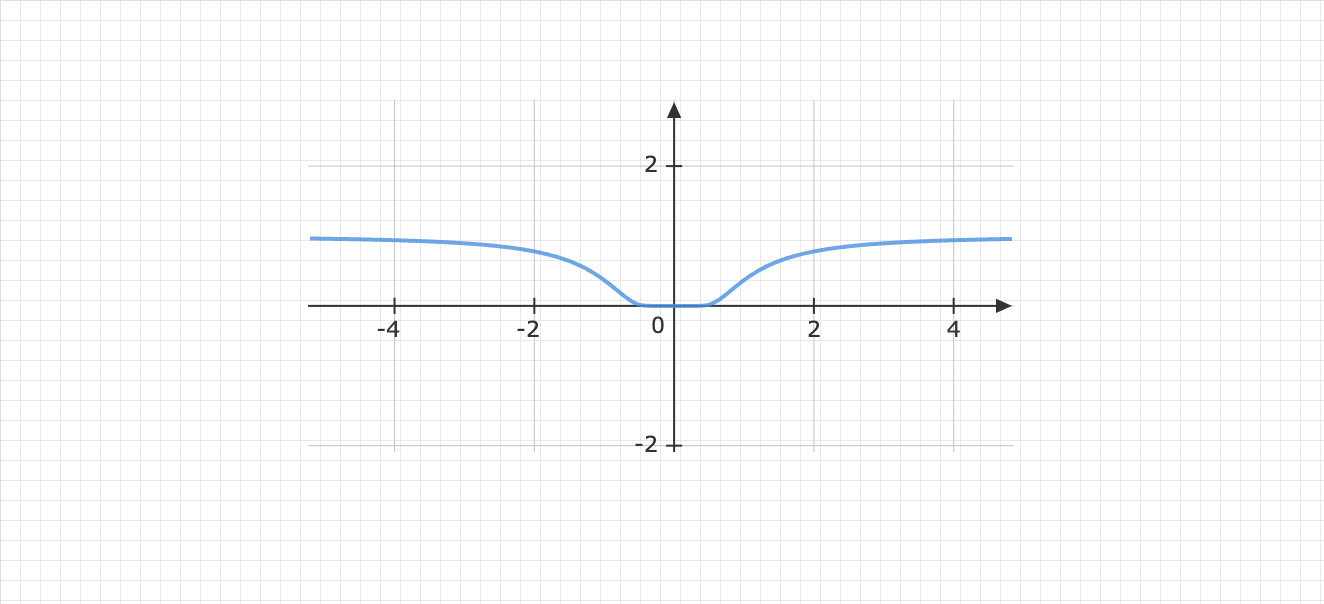
\includegraphics[scale = 0.25]{diagram-20240422 (1).png}
\end{center}
Note that the function is even, so $f(x) = f(-x)$. So, we can shift $f(x) = f(-x)$ by $1$ and $-1$ to see
\begin{center}
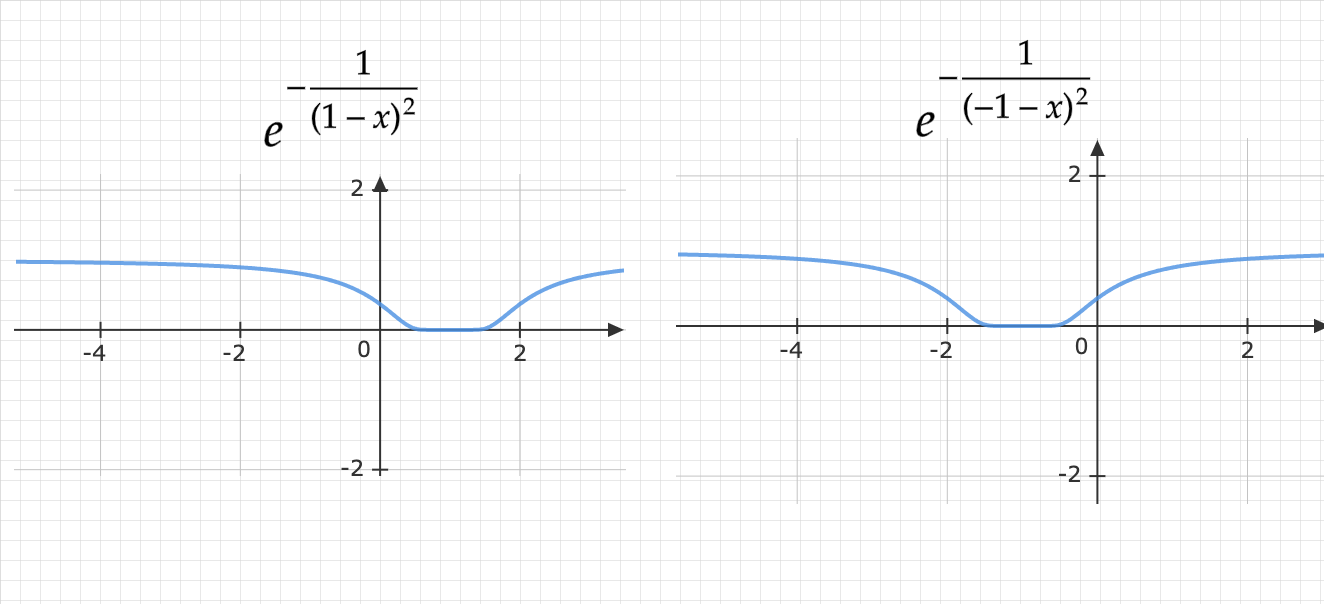
\includegraphics[scale = 0.25]{diagram-20240422.png}
\end{center}
Multiplying the two together we get 
\[
 f(x) = \begin{cases}
  0 , \ x \in \mathbb{R}\backslash(-1, 1)\\
  e^{-\frac{1}{(1 - x)^2}} \cdot e^{-\frac{1}{(-1 - x)^2}}, \ x\in (-1, 1)
 \end{cases} 
\]
with graph 
\begin{center}
  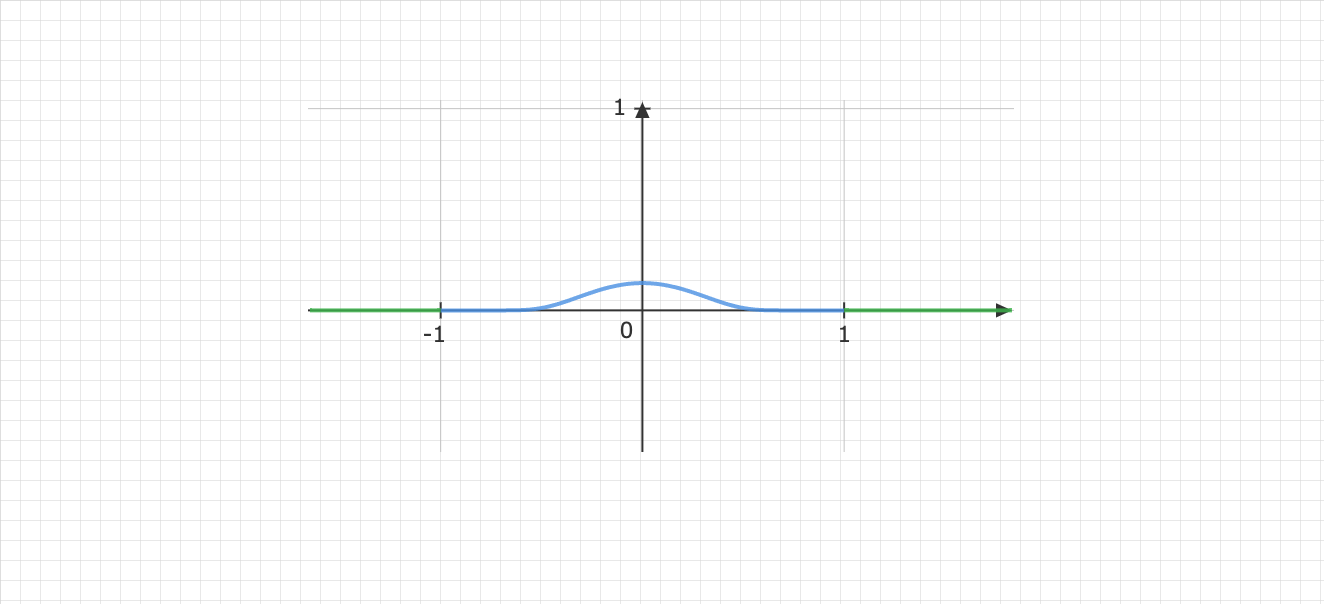
\includegraphics[scale = 0.25]{diagram-20240422 (2).png}
\end{center}
The function is bounded and continuous on $-1$ to $1$ so an integral exists. Then \[
 \frac{1}{C}\int_{-1}^1f(x) = 1 
\]
for $C$ a normalization constant. 
\end{proof}
\section*{5.}
\subsection*{a.}
\begin{proof}
  By change of variables we have \[
  g(x) = \int_{-\infty}^{\infty}f(x - t)p(t)\mathrm{d}t = \int_{-\infty}^{\infty}p(x - t)f(t) \mathrm{d}t.  
  \]
  Using Leibniz integration rule, since $f$ is continuous, we can interchange integral and derivative
  \[
  g'(x) = \frac{d}{dx}\int_{-\infty}^{\infty}p(x - t)f(t) \mathrm{d}t = \int_{-\infty}^{\infty}p(x - t)f(t) \mathrm{d}t  
  \]
  and since $p$ is $C^{\infty}$ we have that 
  \[
  \int_{-\infty}^{\infty}p(x - t)f(t)\mathrm{d}t = \int_{-\infty}^{\infty}f(x - t)p(t)\mathrm{d}t  
  \]
  is differentiable. Since $p$ is $C^{\infty}$, for any higher derivatives
  \[
  g^{(n)}(x) = \frac{d^n}{dx^n} \int_{-\infty}^{\infty}p(x - t)f(t)\mathrm{d}t  
  \]
  we can keep applying the Leibniz integration rule by continuity of $f$ and get 
  \[
  g^{(n)}(x) = 
  int_{-\infty}^{\infty}\frac{d^n}{dx^n}p(x - t)f(t)\mathrm{d}t  
  \]
  and thus as $p$ is $C^{\infty}$, it is $n-\text{times}$ differentiable, implying $g$ is $C^{\infty}$. 
\end{proof}
\subsection*{b.}
\begin{proof}
  Fix $M \in \mathbb{R}$ and $x \in [-M, M]$ and $\epsilon > 0$:
  \begin{align*}
    \left|\int_{-\infty}^{\infty}p_{\epsilon}(t)f(x - t)\mathrm{d}t - f(x) \right| &= \left|\int_{-\infty}^{\infty}p_{\epsilon}(t)f(x - t)\mathrm{d}t - 1 \cdot f(x) \right| \\
    &\numeq{a} \left|\int_{-\infty}^{\infty}p_{\epsilon}(t)f(x - t)\mathrm{d}t - \int_{-\infty}^{\infty}p_{\epsilon}(t)\mathrm{d}t f(x) \right|\\
    &= \left|\int_{-\infty}^{\infty}p_{\epsilon}(t)f(x - t)\mathrm{d}t - \int_{-\infty}^{\infty}p_{\epsilon}(t)f(x)\mathrm{d}t \right| \\
    &= \left|\int_{-\infty}^{\infty}p_{\epsilon}(t)(f(x - t) - f(x))\mathrm{d}t \right| \\
    &\numleq{b}\int_{-\infty}^{\infty}\left|p_{\epsilon}(t)\right||(f(x - t) - f(x))|\mathrm{d}t\\
    &\numleq{c}\delta \int_{-\infty}^{\infty}\left|p_{\epsilon}(t)\right|\mathrm{d}t \\
    &\numeq{d} \delta \int_{-\infty}^{\infty}p_{\epsilon}(t)\mathrm{d}t \\
    &\numeq{e}\delta
  \end{align*}
  which is picked small. Steps $(a)-(e)$ are justified:
  \begin{enumerate}[\indent(a)]
    \item \[
    \int_{-\infty}^{\infty}p_{\epsilon}(t) \mathrm{d}t = 1  
    \]
    \item triangle inequality for integrals
    \item continuity of $f$ allows us to say that $|f(x - t) - f(x)| < \delta$
    \item $p_{\epsilon}(t) > 0$ for all $t \in \mathbb{R}$
    \item \[
      \int_{-\infty}^{\infty}p_{\epsilon}(t) \mathrm{d}t = 1.
    \]
  \end{enumerate}
\end{proof}
\section*{6.}
\begin{proof}
  Let $f:\mathbb{R} \to \mathbb{R}$ be continuous. Define 
  \[
  f_n p_{\frac{1}{n}}(x)*f(x) = \int_{-\infty}^{\infty}p_{\frac{1}{n}}(t)f(x - t)\mathrm{d}t.   
  \]
  By the previous problem, and since $n \to \infty$ we have $\frac{1}{n} \to 0$, we can apply previous result to say 
  \[
  \lim\limits_{n \to \infty}\int_{-\infty}^{\infty}p_{\frac{1}{n}}(t)f(x - t)\mathrm{d}t = f(x).   
  \]
\end{proof}
\section*{7.}
\subsection*{a.}
\begin{proof}
  Beginning with that $D_N(x) = \frac{1}{2 \pi}\frac{\sin\left(\left(N + \frac{1}{2}\right)x\right)}{\sin\left(\frac{1}{2}x\right)}$:
  \begin{align*}
    \int_{-\pi}^{\pi}D_N(x) \mathrm{d}x &= \frac{1}{2 \pi}\int_{-\pi}^{\pi}\frac{\sin\left(\left(N + \frac{1}{2}\right)x\right)}{\sin\left(\frac{1}{2}x \right)}\mathrm{d}x \\
    &\numeq{a}\frac{1}{2 \pi}\int_{-\pi}^{\pi}\sum\limits_{n = -N}^Ne^{inx}\mathrm{d}x \\
    &= \frac{1}{2 \pi }\int_{-\pi}^{\pi}\left(1 + \sum\limits_{n = -N}^{-1}e^{inx} + \sum\limits_{n = 1}^Ne^{inx} \right)\mathrm{d}x \\
    &= \frac{1}{2 \pi }\left(\int_{-\pi}^{\pi} 1\mathrm{d}x + \int_{-\pi}^{\pi}\sum\limits_{n = -N}^{-1}e^{inx} \mathrm{d}x + \int_{-\pi}^{\pi} \sum\limits_{n = 1}^Ne^{inx} \mathrm{dx} \right) \\
    &\numeq{b} \frac{1}{2 \pi}\left(2 \pi + \sum\limits_{n = -N}^{-1}\int_{-\pi}^{\pi}e^{inx}\mathrm{d}x + \sum\limits_{n = 1}^N\int_{-\pi}^{\pi}e^{inx}\mathrm{d}x \right) \\
    &= \frac{1}{2 \pi} \left(2 \pi + \sum\limits_{n = -N}^{-1}\frac{1}{in}\left(e^{in \pi} - e^{-in \pi} \right) + \sum\limits_{n = 1}^N\frac{1}{in}\left(e^{in \pi} - e^{-in\pi} \right)\right) \\
    &\numeq{c} \frac{1}{2 \pi}(2 \pi + 0 + 0) \\
    &= 1
  \end{align*}
  with steps $(a)-(c)$ justified:
  \begin{enumerate}[\indent(a)]
   \item In the book page 37 we the Dirichlet kernel is also equal to \[
    \frac{\sin\left(\left(N + \frac{1}{2}\right)x\right)}{\sin\left(\frac{1}{2}x\right)} = \sum\limits_{n = -N}^Ne^{inx}
   \] 
    \item can interchange finite sum and integral 
    \item \begin{align*}
      e^{in \pi} - e^{-in\pi} &= \cos(n \pi) + i \sin(n \pi) - \cos(-n \pi) - i\sin(-n\pi)\\
      &= \cos(n \pi) - \cos(n \pi) \\
      &= 0.
    \end{align*}
  \end{enumerate}
\end{proof}
\subsection*{b.}
\begin{proof}
  Note, $\left|\sin\left(\frac{x}{2}\right)\right| \leq \left|\frac{x}{2}\right|$, so 
  \[
  |D_N(x)| \geq 2 \frac{\left|\sin\left(\left(N + \frac{1}{2}\right)x\right)\right|}{|x|}.  
  \]
  It follows 
  \begin{align*}
    \frac{1}{2 \pi} \int_{-\pi}^{\pi}|D_N(x)|\mathrm{d}x &\numeq{a}\frac{1}{\pi}\int_0^{\pi}|D_N(x)|\mathrm{d}x \\
    &\leq \frac{2}{\pi}\int_0^{\pi}\frac{\left|\sin\left(\left(N + \frac{1}{2}\right)x\right)\right|}{|x|}\\
    &\numeq{b}\frac{2}{\pi}\int_0^{\left(N + \frac{1}{2}\right)\pi}\frac{|\sin(u)|}{u}\mathrm{d}u \\
    &= \frac{2}{\pi}\sum\limits_{k = 0}^{N - 1}\int_{k \pi}^{(k + 1)\pi} \frac{|\sin(u)|}{u}\mathrm{d}u + \frac{2}{\pi}\int_{N \pi}^{\left(N + \frac{1}{2}\right)\pi}\frac{|\sin(u)|}{u}\mathrm{d}u \\
    &\geq \frac{2}{\pi}\sum\limits_{k = 0}^{N - 1}\int_{k \pi}^{(k + 1)\pi} \frac{|\sin(u)|}{(k + 1)\pi}\mathrm{d}u + \frac{2}{\pi}\int_{N \pi}^{\left(N + \frac{1}{2}\right)\pi}\frac{|\sin(u)|}{\left(N + \frac{1}{2}\right)\pi}\mathrm{d}u \\
    &\numeq{c} \frac{2}{\pi^2} \sum\limits_{k = 0}^{N - 1}\int_{k \pi}^{(k + 1)\pi} \frac{|\sin(u)|}{(k + 1)}\mathrm{d}u + O(1) \\
    &= \frac{2}{\pi^2}\sum\limits_{k = 0}^{N - 1}\frac{1}{k + 1}\left[|\cos(u)|\right]_{k \pi}^{(k + 1)\pi} + O(1) \\
    &= \frac{2}{\pi^2}\sum\limits_{k = 0}^{N - 1}\frac{1}{k + 1}\cdot 2 + O(1)\\
    &= \frac{4}{\pi^2}\sum\limits_{k = 1}^N\frac{1}{k}+ O(1) \\
    &\numgeq{d}\frac{4}{\pi^2}\cdot C \log(N) + O(1) \xrightarrow[N \to \infty]{}\infty
  \end{align*}
  because $\log(N) \to infty$ as $N\to \infty$.
  The steps $(a)-(d)$ are justified:
  \begin{enumerate}[\indent(a)]
    \item even function
    \item change of variables, take $u= \left(N + \frac{1}{2}\right)x$ and $\frac{du}{dx} = N + \frac{1}{2}$
    \item $\frac{2}{\pi}\int_{N \pi}^{\left(N + \frac{1}{2}\right)\pi}\frac{|\sin(u)|}{\left(N + \frac{1}{2}\right)\pi}\mathrm{d}u$ is $O(1)$
    \item hint given in book that
    \[
    \sum\limits_{k = 1}^n\frac{1}{k} \geq c \log(n).  
    \]
  \end{enumerate} 
  Thus, 
  \[
  \lim\limits_{N \to \infty} \int_{-\pi}^{\pi}|D_N(x)|\mathrm{d}x \to \infty.
  \]
\end{proof}
\end{document}
